\chapter{Requirements of the system}
\label{chap:systemanforderungen}

The following sections deal with the requirements of the system. Functional and non-functional requirements will be defined. Section \ref{subsec:af-tabelle} in the appendix also contains an overview in tabular form. The functionalities that are required and desired are thereby described with the aid of use case diagrams. This chapter will provide an answer to the question of what a system has to provide for it to fulfil the requirements set in the analysis (chapter \ref{chap:analyse}).


\section{Functional requirements}
\label{sec:funktionale-af}

\subsection{Must-haves}
\label{subsec:muss}

Figure \ref{fig:usecasediagramm-muss-editor} depicts a use case diagram for the requirements of the outline management and the outliner that were identified as strictly necessary. Figure \ref{fig:usecasediagramm-muss-repl} depicts the requirements of replication and conflict resolution. The prototype to be developed in this thesis must meet these requirements. Only then the implementation of the task may be called successful.

\medskip
\begin{figure}[ht] 
  \begin{center}
  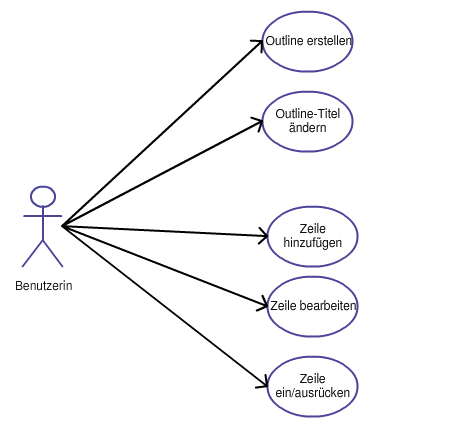
\includegraphics[width=0.6\textwidth]{grafik/usecasediagramm-muss-editor} 
  \end{center}
  \caption{Use case diagram for the requirements of outline management}
  \label{fig:usecasediagramm-muss-editor} 
\end{figure}

\medskip
\begin{figure}[ht] 
  \begin{center}
  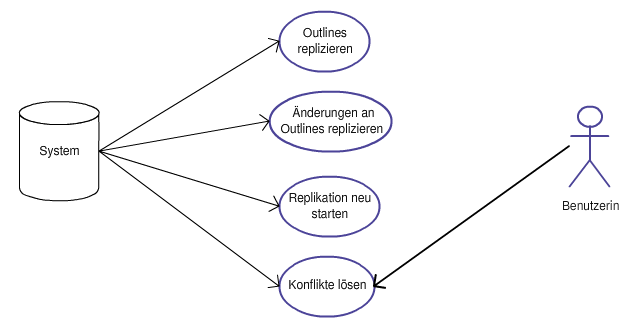
\includegraphics[width=\textwidth]{grafik/usecasediagramm-muss-repl} 
  \end{center}
  \caption{Use case diagram for the requirements of replication}
  \label{fig:usecasediagramm-muss-repl} 
\end{figure}

\subsubsection{Outline management}

The user should be able to create any number of outlines (\textbf{FA100}). The outlines should be clearly represented and their title should be changeable (\textbf{FA101}). 

\subsubsection{Outliner}
\label{subsec:gliederungseditor}

The outliner is to have the look \& feel of a text editor with an unlimited number of lines (\textbf{FA200}). It should be possible to navigate between the lines using (combinations of) keystrokes (\textbf{FA201}). The contents of the lines should be editable (\textbf{FA202}). When the cursor leaves a line it should automatically be saved (\textbf{FA203}). When the window is closed while editing a line it should be automatically saved. Alternatively, before closing the window the user should be informed about the possible loss of data (\textbf{FA206}).

The lines have to be able to indent and outdent in order to represent the underlying hierarchy (\textbf{FA204}). Indenting or outdenting a line should immediately move any following lines that are at a deeper indentation level (\textbf{FA205}).

\subsubsection{Replication}

If the user is on-line or if the connection is restored after an off-line period, the outlines (\textbf{FA300}) and changes to outlines (\textbf{FA301}) made by the user should immediately be replicated to the server.

Outlines (\textbf{FA302}) and changes to outlines (\textbf{FA303}) should automatically and immediately be replicated to the user's computer while they are connected to the server. The user must be informed about changes as soon as they arise (\textbf{FA304}) without interrupting the user's work.

If the connection is restored after an off-line period, the user should either be informed that replication is again possible, or replication should start automatically (\textbf{FA305}).

\subsubsection{Conflict handling}

Of the conflicts that may arise during replication, at least one type should be resolved automatically by the system (\textbf{FA400}). At least one conlict type should be resolved manually (\textbf{FA401}).

\subsection{May-haves}
\label{subsec:kann}

Not all criteria listed in this section must be implemented in the prototype. Their later implementation should, however, be taken in consideration during the design phase.

Figure \ref{fig:usecasediagramm-kann-editor} depicts a use case diagram for the requirements of outline management and the outliner that were identified as optional. Figure \ref{fig:usecasediagramm-kann-repl} illustrates the requirements of replication and conflict resolution.

\medskip
\begin{figure}[ht] 
  \begin{center}
  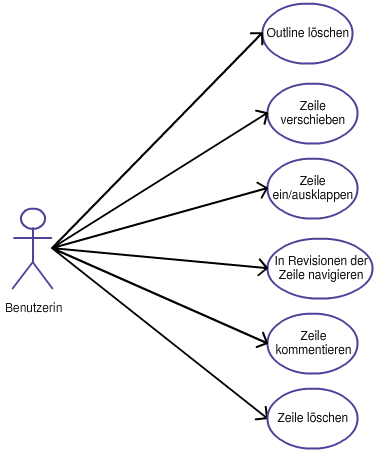
\includegraphics[width=0.6\textwidth]{grafik/usecasediagramm-kann-editor} 
  \end{center}
  \caption{Use case diagram for optional requirements, outline management}
  \label{fig:usecasediagramm-kann-editor}
\end{figure}

\medskip
\begin{figure}[ht] 
  \begin{center}
  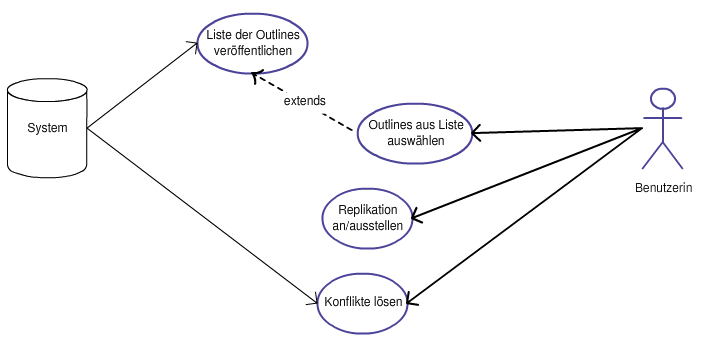
\includegraphics[width=\textwidth]{grafik/usecasediagramm-kann-repl} 
  \end{center}
  \caption{Use case diagram for optional requirements, replication}
  \label{fig:usecasediagramm-kann-repl} 
\end{figure}


\subsubsection{Outline management}

It should be possible to delete outlines (\textbf{FA102}).

\subsubsection{Outliner}

It should be possible to move lines up or down (\textbf{FA207}). Their size should automatically adapt to the amount of text (\textbf{FA208}). To increase clarity, it should be possible to collapse or expand the lines (\textbf{FA209}). Information about which lines have been collapsed should not be replicated but possibly locally stored (\textbf{FA210}).

The revision of a line should be saved automatically (\textbf{FA211}). The user should be able to jump between revisions (\textbf{FA212}). It should be possible to add comments to individual lines (\textbf{FA213}) and to remove the lines (\textbf{FA214}).

\subsubsection{Replication}

The available outlines should be published by the system so that connected users may choose which single outlines they want to replicate (\textbf{FA306}).

The user should be notified whether a connection to the server is established (\textbf{FA307}). The interface should allow replication to be activated and deactivated (\textbf{FA308}).

\subsubsection{Conflict resolution}

Combinations of multiple conflict types should be solvable by the system or the user (\textbf{FA402}). Conflicts that occur between more than two replicas should be treated correctly (\textbf{FA403}).

The system should be able to independently resolve as many conflicts as possible (\textbf{FA404}). The interface should be developed so that the user might resolve as many conflict types as possible by hand (\textbf{FA405}).


\subsection{Demarcation criteria}

\subsubsection{Outline management}

No user or access management will be implemented for outlines.

\subsubsection{Outliner}

No columns will be implemented.

\subsubsection{Replication}

No peer-to-peer replication will be implemented.

\subsubsection{Conflict resolution}

The system will only be optimised for use by a lesser number of users. For conflicts between more than two versions there may be no reliable conflict resolution.

\section{Non-functional requirements}

\subsection{Usage}
\label{subsec:einsatz}

\subsubsection{Target audience}

Users of the system should have average knowledge of how to use computers and web browsers in particular. Furthermore, they should be able to install and run a CouchDB instance on their computer. The users should have some understanding of the advantages and restrictions of using such a system.

\subsubsection{Operating conditions}

The server responsible for exchanging outlines and updates should be able to run 24 hours per day and seven days a week in order for the services to remain available at all times. To ensure this, the service should be deployed using Amazon's Elastic Compute Cloud (Amazon EC2) service. Greater scalability is achieved with the aid of the clustering framework CouchDB Lounge.

The application should run on every computer capable of running CouchDB. Further information about systems supported by CouchDB can be found in section \ref{sec:installation}.


\subsection{Environment}

In order to avoid licence fees and to be able to adapt the system to varying demands, it should exclusively be implemented using open-source software.


\subsubsection{Hardware}

Should the CouchDB instance that has the server role not run on Amazon EC2, but rather on a private server, this server should meet at least the following system requirements:

\begin{itemize}  
  \item[-] Intel processor clocked at 3,0 GHz
  \item[-] 5 GB of free disk space
  \item[-] 1 GB RAM memory
  \item[-] Ethernet connection of 100 MBit
\end{itemize}


\subsubsection{Software}

The system is built on several software packages and programming languages. The versions indicated are the minimum requirements. Installation notes can be found in section \ref{sec:installation}.

\begin{itemize}  
  \item[-] CouchDB 0.11.0
  \item[-] Spidermonkey 1.7
  \item[-] Erlang 5.6.5
  \item[-] ICU 3.0
  \item[-] cURL 7.18.0
  \item[-] Automake 1.6.3
  \item[-] Autoconf 2.59
\end{itemize}

The Rake tasks supplied for deployment and operation require Ruby version 1.8.6 or higher to run (see section \ref{subsec:hilfestellung}).

Section \ref{sec:systemtest} contains some notes regarding the test set-up.

\subsection{User interface}
\label{subsec:gui-anf}

The system requires a simple and transparent web interface. It is assumed that the user has JavaScript activated. The user interface should run without restrictions in Firefox 3.5 or newer. The optimal delay between input via the web interface and the activation of the desired function is under one second and should in no case exceed four seconds. This time span is the reaction time that people tolerate in normal conversation or telephone systems \citelit[p. 267 \& 270]{response:miller}. Jakob Nielsen connects this time span to interaction times in web applications \citelit[chap. 5.5]{nielsen:response}.

Figure \ref{fig:interface-mockup-list} depicts a mock-up for the interface showing the outline overview. Figure \ref{fig:interface-mockup} shows the structure of the site containing the outliner.

\medskip
\begin{figure}[ht] 
  \begin{center}
  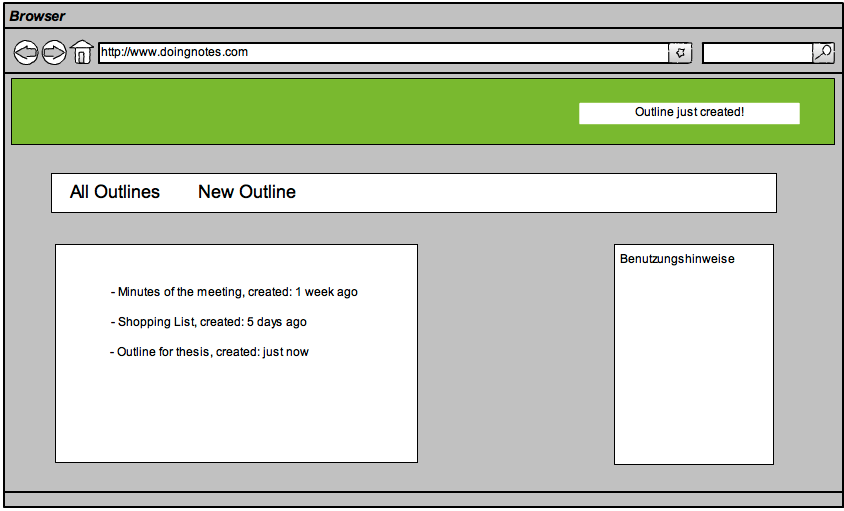
\includegraphics[width=\textwidth]{grafik/user-interface-mockup-list} 
  \end{center}
  \caption{Layout of the web interface: outline overview}
  \label{fig:interface-mockup-list} 
\end{figure}

\medskip
\begin{figure}[ht] 
  \begin{center}
  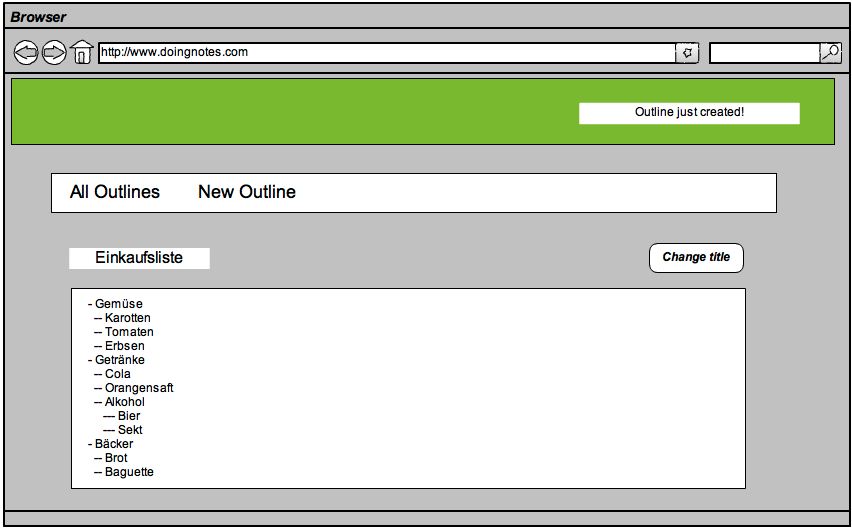
\includegraphics[width=\textwidth]{grafik/user-interface-mockup} 
  \end{center}
  \caption{Structure of the web interface: single outline view}
  \label{fig:interface-mockup} 
\end{figure}


\subsection{Quality goals}

The quality of the final system is another important goal. The following quality requirements have to be respected:

\begin{itemize}  
  \item Expandability through open architecture
  \item Portability through low hardware and software requirements
  \item High software quality through extensive testing
  \item Design and programming after framework-specific standards
  \item Implementation according to the MVC architecture: separation of interface, application logic and data
  \item Highly maintainable and therefore simple and non-redundant code
  \item Adherence to usability and accessibility guidelines with regard to the interface
  \item Fast-loading application and therefore little dependency on external frameworks
\end{itemize}